\documentclass[11pt,aspectratio=169]{beamer}

\usetheme{Madrid}
\usecolortheme{default}

\definecolor{guardian}{RGB}{245,158,11}
\definecolor{darkbg}{RGB}{17,24,39}
\definecolor{codegreen}{RGB}{16,185,129}

\setbeamercolor{structure}{fg=guardian}
\setbeamercolor{palette primary}{bg=darkbg, fg=white}
\setbeamercolor{palette secondary}{bg=darkbg!90, fg=white}
\setbeamercolor{palette tertiary}{bg=guardian!90!black, fg=white}
\setbeamercolor{frametitle}{bg=darkbg, fg=white}
\setbeamercolor{title}{bg=darkbg, fg=white}
\setbeamercolor{block title}{bg=guardian!15, fg=darkbg}
\setbeamertemplate{navigation symbols}{}
\setbeamertemplate{footline}[frame number]

\usepackage{booktabs}
\usepackage{graphicx}
\usepackage{tikz}
\usetikzlibrary{arrows.meta, positioning}
\graphicspath{{screenshots/}}

\title{TrustChain-AI}
\subtitle{Software Supply Chain Guardian\\[2pt]
\small Know What You Build. Trust What You Ship.}
\author{Bosch BGSW Hackathon}
\date{November 2026}

\begin{document}

% ---------------------------------------------------------------- 1
\begin{frame}
\titlepage
\begin{center}
\small Deterministic tools produce facts. Gemini agents only reason, explain and prioritize.
\end{center}
\end{frame}

% ---------------------------------------------------------------- 2
\begin{frame}{The problem}
\begin{columns}[T]
\begin{column}{0.62\textwidth}
\begin{itemize}
  \item \textbf{Visibility:} thousands of transitive dependencies, opaque provenance.
  \item \textbf{Noise:} severity $\neq$ risk — an unreached critical CVE is less urgent than a reached high one.
  \item \textbf{Trust:} CVE scanners miss supply-chain attacks: typosquats, malicious packages, unpinned CI actions, unsafe install scripts.
\end{itemize}
\end{column}
\begin{column}{0.34\textwidth}
\begin{block}{Required workflow}
\small Discover $\rightarrow$ Detect $\rightarrow$ Analyze $\rightarrow$ Remediate (human approval) $\rightarrow$ Validate
\end{block}
\end{column}
\end{columns}
\end{frame}

% ---------------------------------------------------------------- 3
\begin{frame}{Architecture: facts and reasoning never mix}
\begin{center}
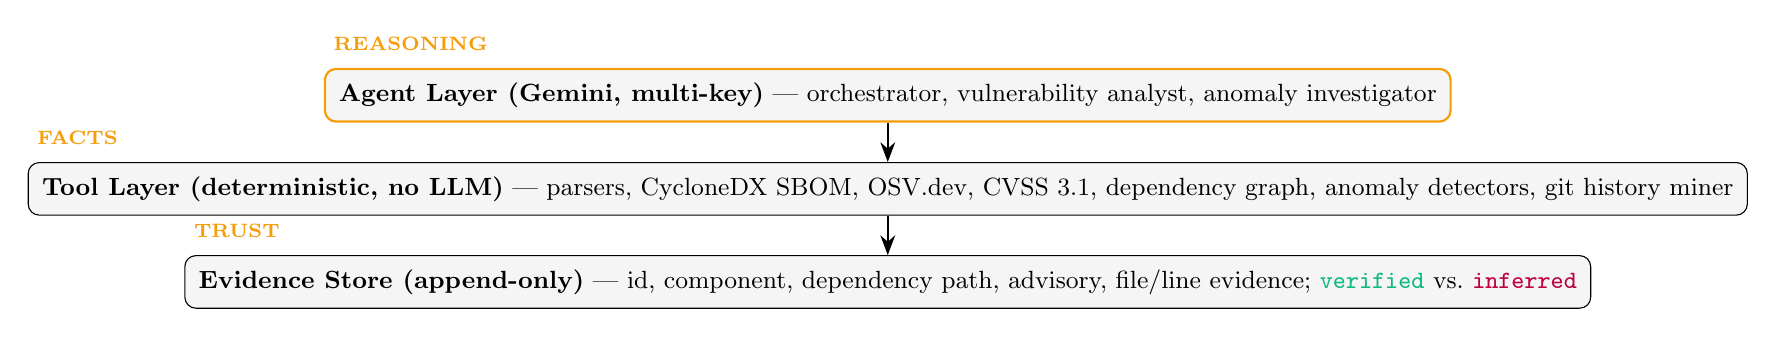
\begin{tikzpicture}[
  node distance=5mm,
  box/.style={draw, rounded corners, fill=gray!8, minimum width=13.2cm, align=center, inner sep=5pt},
  layer/.style={font=\bfseries\scriptsize, text=guardian},
  arr/.style={-{Stealth[length=2.5mm]}, thick}
]
\node[box, draw=guardian, thick] (agent) {
  \small \textbf{Agent Layer (Gemini, multi-key)} — orchestrator, vulnerability analyst, anomaly investigator};
\node[layer, above=1mm of agent.north west, anchor=south west] {REASONING};
\node[box, below=5mm of agent] (tools) {
  \small \textbf{Tool Layer (deterministic, no LLM)} — parsers, CycloneDX SBOM, OSV.dev, CVSS 3.1,
  dependency graph, anomaly detectors, git history miner};
\node[layer, above=1mm of tools.north west, anchor=south west] {FACTS};
\node[box, below=5mm of tools] (evidence) {
  \small \textbf{Evidence Store (append-only)} — id, component, dependency path, advisory, file/line
  evidence; \textcolor{codegreen}{\texttt{verified}} vs.\ \textcolor{purple}{\texttt{inferred}}};
\node[layer, above=1mm of evidence.north west, anchor=south west] {TRUST};
\draw[arr] (agent) -- (tools);
\draw[arr] (tools) -- (evidence);
\end{tikzpicture}
\end{center}
\end{frame}

% ---------------------------------------------------------------- 4
\begin{frame}{Why agents cannot hallucinate findings}
\begin{enumerate}
  \item \textbf{Stable identifiers:} every finding enters the agent layer with an id (T-0001, \dots) from the evidence ledger.
  \item \textbf{Contract prompts:} agents must return one JSON object using \emph{only} the given ids.
  \item \textbf{Id-filtered merge:} the orchestrator discards any key not in the input set; malformed or truncated output is dropped entirely.
\end{enumerate}
\begin{block}{Result}
AI text can only \emph{annotate} tool-verified facts — never create, delete, or alter them.
\end{block}
\end{frame}

% ---------------------------------------------------------------- 5
\begin{frame}{Day 1 pipeline (fully working)}
\begin{enumerate}
  \item \textbf{Discover:} npm lockfile v2/v3, Yarn classic + Berry, pip manifests.
  \item \textbf{SBOM:} CycloneDX 1.5 with purls, licenses, hashes.
  \item \textbf{Graph:} dependency graph + reverse dependencies.
  \item \textbf{CI/CD \& containers:} workflows, Dockerfiles, lifecycle scripts.
  \item \textbf{CVEs:} OSV.dev correlation + CVSS 3.1 + path tracing.
  \item \textbf{Anomalies:} 5 non-CVE detectors.
  \item \textbf{Report:} agents + evidence ledger $\rightarrow$ Guardian Report.
\end{enumerate}
\begin{center}
\small Scan any public GitHub URL in the web UI — live 7-step checklist.
\end{center}
\end{frame}

% ---------------------------------------------------------------- 6
\begin{frame}{Discovery and supply-chain view (Strapi)}
\begin{columns}[T]
\begin{column}{0.5\textwidth}
\begin{itemize}
  \item \textbf{3002} components discovered: 412 direct, 2590 transitive.
  \item CycloneDX 1.5 SBOM with full purl set.
  \item Dependency graph: \textbf{3003 nodes / 7126 edges}.
  \item CI/CD workflows, Dockerfiles, install scripts inspected.
\end{itemize}
\end{column}
\begin{column}{0.5\textwidth}
\begin{figure}
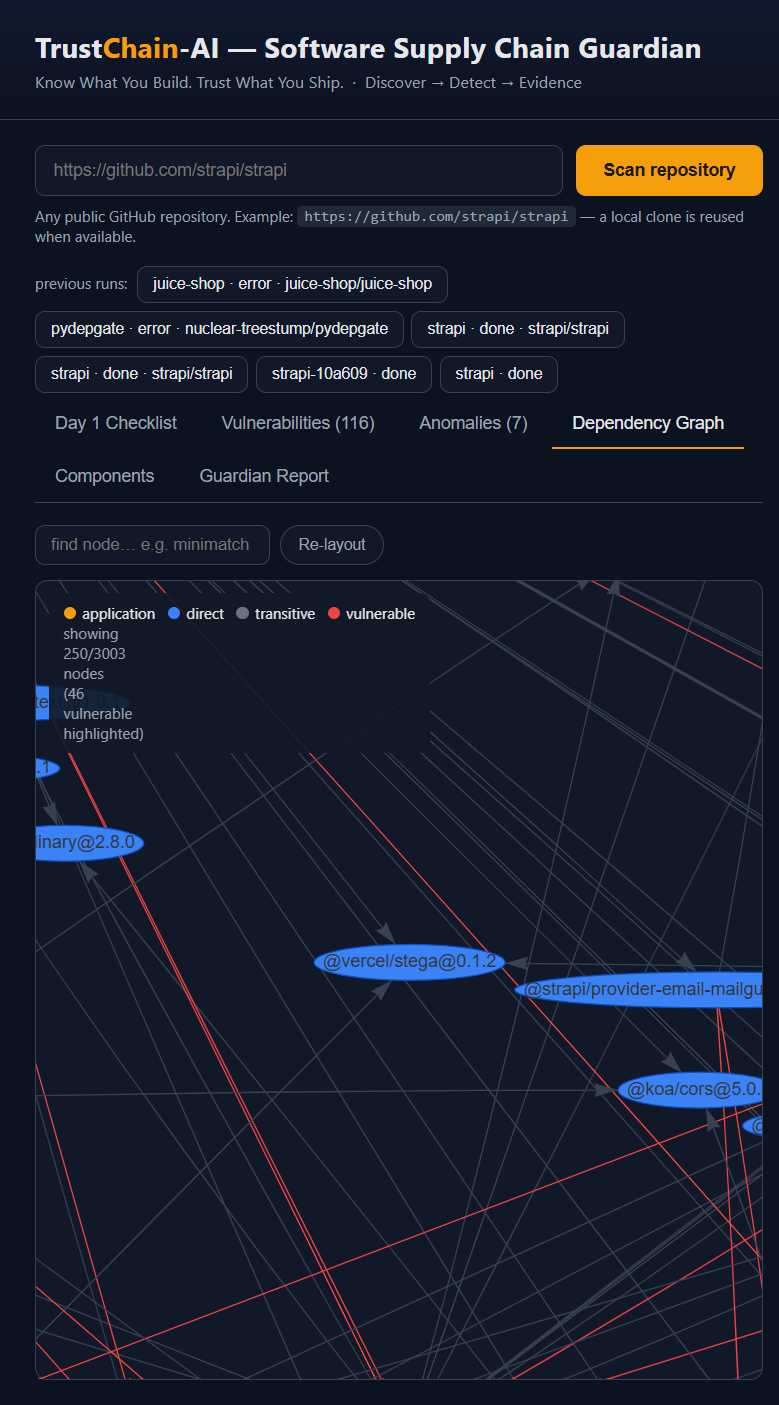
\includegraphics[width=\textwidth,height=0.75\textheight,keepaspectratio]{03-graph.png}
\caption{Vulnerable components highlighted in red.}
\end{figure}
\end{column}
\end{columns}
\end{frame}

% ---------------------------------------------------------------- 7
\begin{frame}{Vulnerability detection}
\begin{columns}[T]
\begin{column}{0.42\textwidth}
\begin{itemize}
  \item OSV.dev batch queries (500/request, shared disk cache).
  \item Severity from the \textbf{CVSS 3.1 vector}, not upstream labels.
  \item Fixed versions extracted from advisory ranges.
  \item Every finding \textbf{traced to its root} via shortest dependency paths.
\end{itemize}
\end{column}
\begin{column}{0.56\textwidth}
\begin{figure}
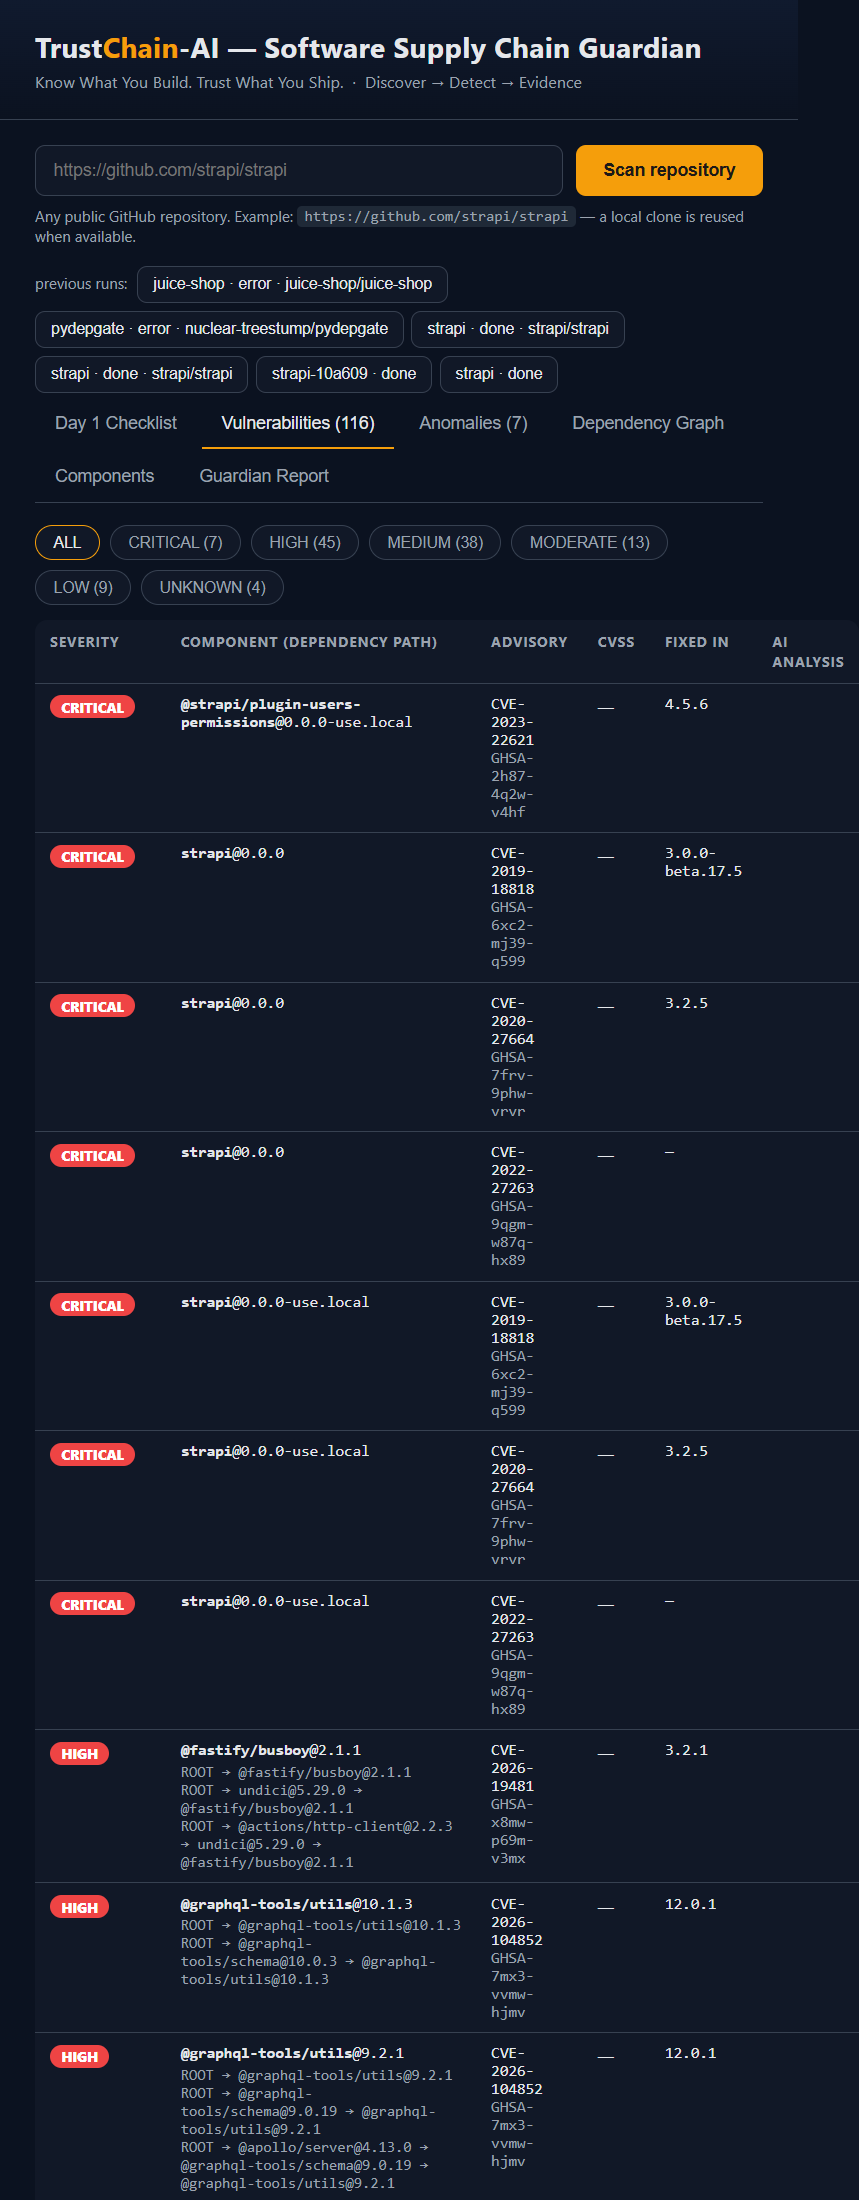
\includegraphics[width=\textwidth,height=0.75\textheight,keepaspectratio]{02-vulnerabilities.png}
\end{figure}
\end{column}
\end{columns}
\end{frame}

% ---------------------------------------------------------------- 8
\begin{frame}{Detection results (Strapi)}
\begin{center}
\begin{tabular}{@{}ll@{}}
\toprule
\textbf{Metric} & \textbf{Value} \\
\midrule
Vulnerability findings & \textbf{116} — 7 critical, 45 high, 38 medium, \dots \\
Malicious-package advisories & \textbf{2} (MAL-2026-1487, MAL-2026-1492) \\
Findings with dependency paths & 56 \\
Non-CVE anomalies & 7 typosquat candidates \\
Evidence ledger & 123 entries (116 verified / 7 inferred) \\
\bottomrule
\end{tabular}
\end{center}
\begin{block}{Key point}
The 2 MAL- advisories are exactly the supply-chain attack class that CVE-only scanners miss.
\end{block}
\end{frame}

% ---------------------------------------------------------------- 9
\begin{frame}{Non-CVE anomaly detection}
\begin{center}
\small
\begin{tabular}{@{}lll@{}}
\toprule
\textbf{Detector} & \textbf{Signals} & \textbf{Confidence} \\
\midrule
CI pinning & \texttt{uses:} not SHA-pinned, \texttt{curl | sh}, \texttt{pull\_request\_target} & verified \\
Container images & \texttt{:latest} tags, unpinned digests & verified \\
Install scripts & risky pre/post-install hooks & verified \\
Typosquat & Levenshtein $\le 2$ to popular names & inferred \\
Lockfile diff & removed/added versions between snapshots & verified \\
\bottomrule
\end{tabular}
\end{center}
\begin{center}
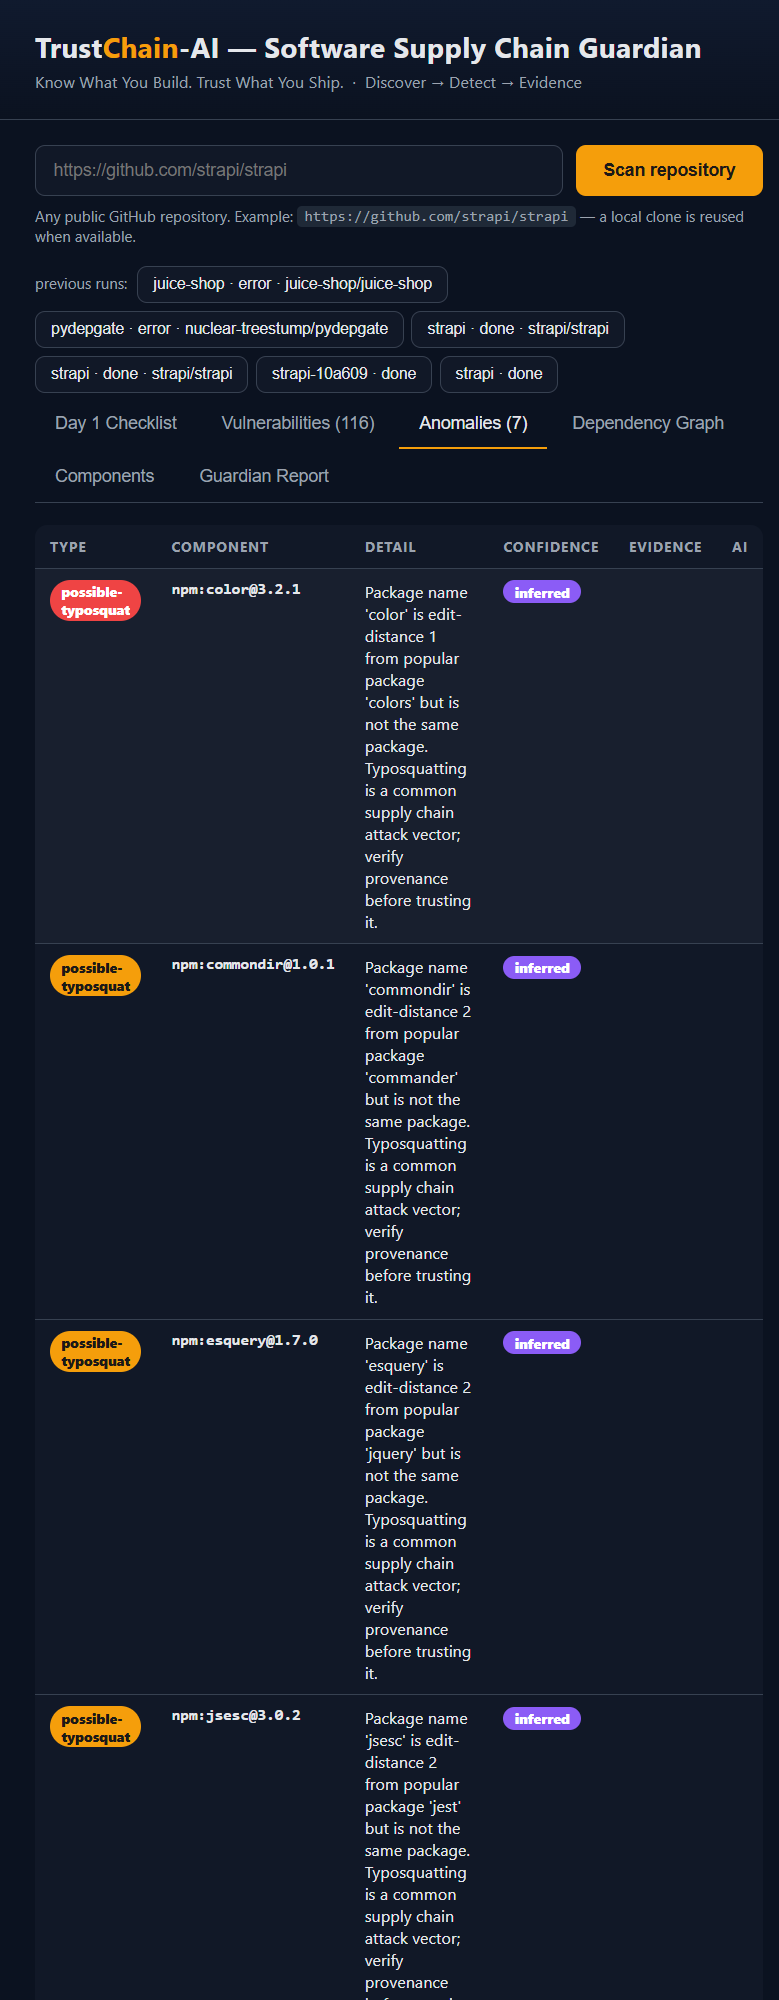
\includegraphics[width=0.55\textwidth,height=0.42\textheight,keepaspectratio]{04-anomalies.png}
\end{center}
\end{frame}

% ---------------------------------------------------------------- 10
\begin{frame}{Gemini multi-key agent client}
\begin{itemize}
  \item Up to \textbf{6 keys} in a git-ignored \texttt{.env} (\texttt{GEMINI\_API\_KEY\_1..6}).
  \item \textbf{429 / 503 / timeouts} $\rightarrow$ rotate to the next key and retry.
  \item Model globally unavailable $\rightarrow$ \textbf{model fallback}: gemini-3.8-flash $\rightarrow$ 3.5-flash $\rightarrow$ 2.5-flash.
  \item Everything fails $\rightarrow$ \textbf{graceful degradation} to a tools-only report; a scan never fails because the LLM is down.
  \item Findings processed in \textbf{batches of 25} so responses never truncate.
\end{itemize}
\end{frame}

% ---------------------------------------------------------------- 11
\begin{frame}{Agents and the human approval gate}
\begin{center}
\small
\begin{tabular}{@{}p{3.4cm}p{4.4cm}p{6cm}@{}}
\toprule
\textbf{Agent} & \textbf{Input} & \textbf{Output per finding id} \\
\midrule
Vulnerability Analyst & verified CVE findings + paths & risk level, attention reason, reachability, confidence \\
Anomaly Investigator & detector output + evidence & verdict, reasoning, action, confidence \\
Orchestrator (deterministic) & artifacts + agent output & evidence ledger, id-filtered merge, report \\
\bottomrule
\end{tabular}
\end{center}
\begin{block}{Responsible AI by construction}
No code path writes to the scanned repository. Remediation (Day 2) requires a human to
approve a proposed change before it is applied on a branch.
\end{block}
\end{frame}

% ---------------------------------------------------------------- 12
\begin{frame}{Retrospective validation}
\small \textit{``How do you know the agent isn't making things up?''} — Strapi's dependabot CVE-fix history is the ground truth:
\begin{enumerate}
  \item Mine \texttt{chore(deps): bump X from A to B} commits (12 analyzed).
  \item Ground truth: advisories that disappear across the bump = confirmed fix (6 of 12).
  \item Rewind to the pre-fix snapshot (\texttt{git worktree}), scan \emph{blind} to the future fix.
  \item Score detections.
\end{enumerate}
\begin{center}
\begin{tabular}{@{}lcc@{}}
\toprule
\textbf{Capability} & \textbf{Result} & \textbf{Recall} \\
\midrule
Vulnerability detection on pre-fix snapshots & 6/6 & \textbf{1.00} \\
Dependency version-change detection & 11/12 & \textbf{0.917} \\
\bottomrule
\end{tabular}
\end{center}
\end{frame}

% ---------------------------------------------------------------- 13
\begin{frame}{Web application}
\begin{columns}[T]
\begin{column}{0.46\textwidth}
\begin{itemize}
  \item Paste any public GitHub URL $\rightarrow$ scan runs in a background thread.
  \item Live Day 1 checklist with per-step details and artifacts.
  \item Findings browser with severity filters.
  \item Interactive graph, components explorer, inline Guardian Report.
  \item Flask + waitress; deployed on Render (blueprint in \texttt{render.yaml}).
\end{itemize}
\end{column}
\begin{column}{0.52\textwidth}
\begin{figure}
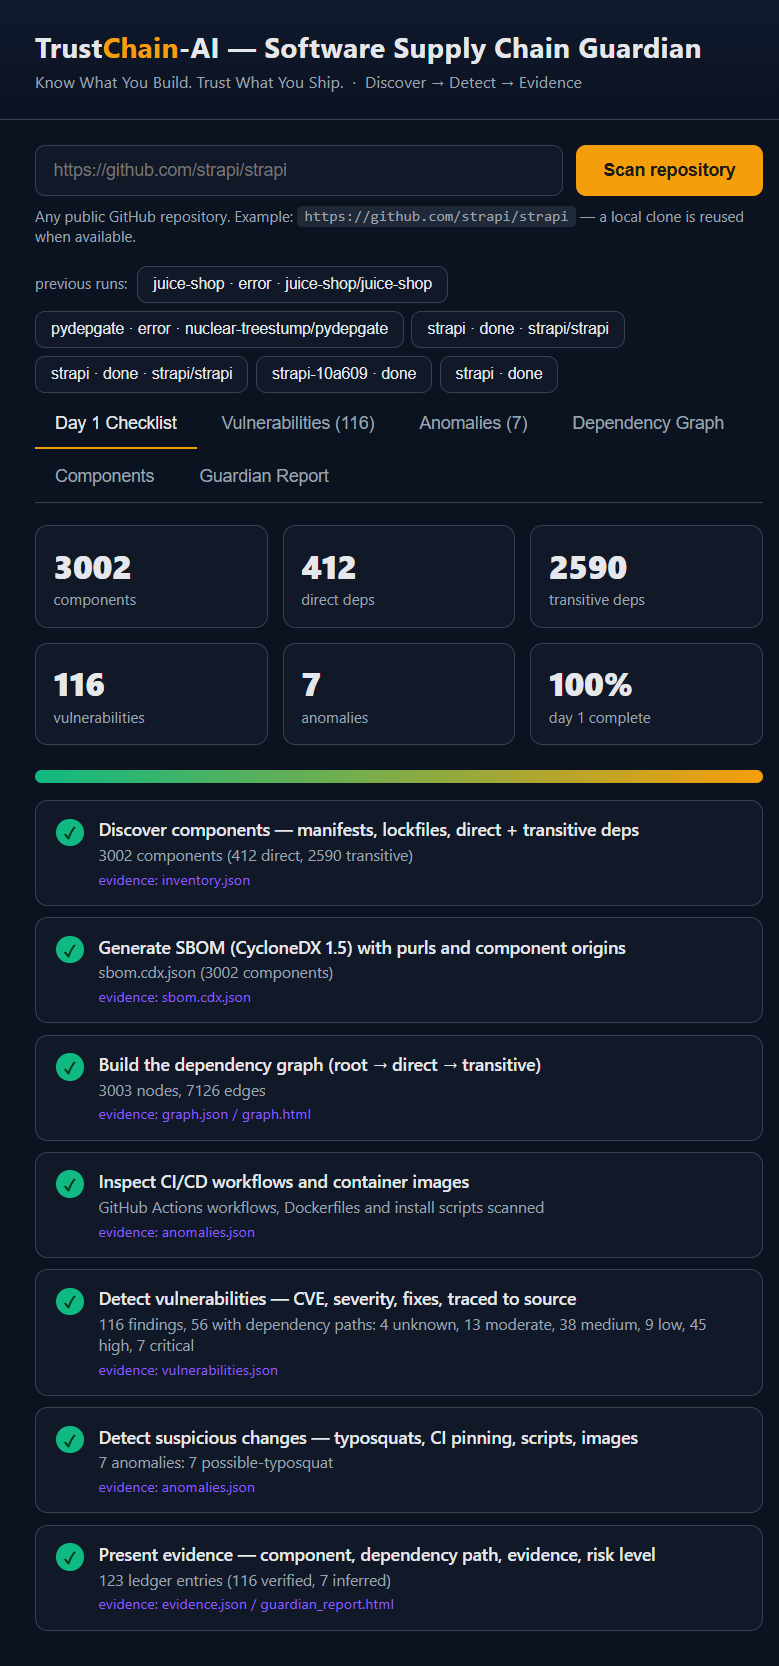
\includegraphics[width=\textwidth,height=0.78\textheight,keepaspectratio]{01-checklist.png}
\caption{Completed Strapi scan, 7/7 steps.}
\end{figure}
\end{column}
\end{columns}
\end{frame}

% ---------------------------------------------------------------- 14
\begin{frame}{Guardian report}
\begin{columns}[T]
\begin{column}{0.52\textwidth}
\begin{figure}
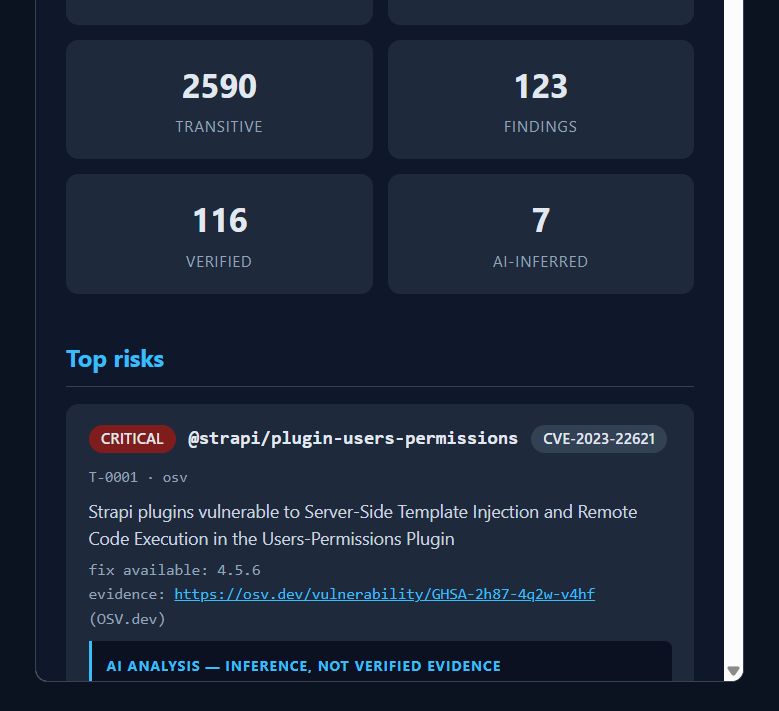
\includegraphics[width=\textwidth,height=0.78\textheight,keepaspectratio]{05-report.png}
\end{figure}
\end{column}
\begin{column}{0.44\textwidth}
\begin{itemize}
  \item Human \emph{and} machine readable (HTML + JSON).
  \item Top-risk cards with dependency paths and fixed versions.
  \item AI blocks labelled \textbf{``inference, not verified evidence''}.
  \item Full methodology and evidence policy.
\end{itemize}
\end{column}
\end{columns}
\end{frame}

% ---------------------------------------------------------------- 15
\begin{frame}{Summary and roadmap}
\begin{columns}[T]
\begin{column}{0.55\textwidth}
\begin{itemize}
  \item Full Day 1 pipeline: discovery $\rightarrow$ SBOM $\rightarrow$ graph $\rightarrow$ CVEs $\rightarrow$ anomalies $\rightarrow$ evidence $\rightarrow$ report.
  \item Validation recall \textbf{1.00 / 0.917} against real fix history.
  \item 42 automated tests passing; 13 milestone commits.
  \item Working web app + Render deployment blueprint.
\end{itemize}
\end{column}
\begin{column}{0.42\textwidth}
\begin{block}{Day 2 roadmap}
Prioritization $\rightarrow$ remediation proposals $\rightarrow$ human-approved branch fix $\rightarrow$ build/test/rescan $\rightarrow$ before/after SBOM diff
\end{block}
\end{column}
\end{columns}
\begin{center}
\textbf{Know What You Build. Trust What You Ship.}\\
\small github.com/saiakhilesh5/TrustChain-AI
\end{center}
\end{frame}

\end{document}
